\documentclass[tikz]{standalone}
\usetikzlibrary{positioning}
\begin{document}
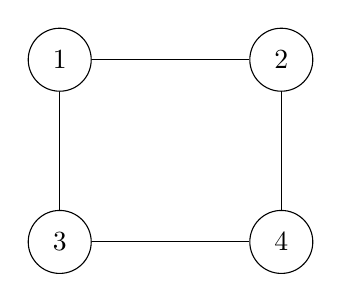
\begin{tikzpicture}[
  node/.style={circle, draw, minimum size=8mm}
]
  \node[node] (n1) {1};
  \node[node, right=2cm of n1] (n2) {2};
  \node[node, below=1.5cm of n1] (n3) {3};
  \node[node, below=1.5cm of n2] (n4) {4};

  \draw (n1) -- (n2);
  \draw (n1) -- (n3);
  \draw (n2) -- (n4);
  \draw (n3) -- (n4);
\end{tikzpicture}
\end{document}
